\section{Acidentes em Braga no ano de 2019}

% todo este conteudo, ate a proxima subsection, corresponde, na pratica,
% à componente de Business Understanding do CRISP-DM
Segundo a PORDATA\footnote{\url{https://www.pordata.pt/Portugal/Acidentes+de+via\%c3\%a7\%c3\%a3o+com+v\%c3\%adtimas++feridos+e+mortos+++Continente-326}}, no ano de 2018, em Portugal, foram registados $34235$ acidentes rodoviários com vítimas, totalizando $508$ vítimas mortais. Como tal, a motivação para o desenvolvimento de um trabalho deste tipo é imediata.

Ao conseguirmos compreender melhor os factores que causam acidentes, trabalhando em específico com os dados da zona de Braga, pretendemos ser capazes de generalizar e compreender quais atributos são os mais informativos no sentido de prever o número de acidentes num determinado dia.

Com um modelo capaz de efectivamente utilizarmos os atributos mais informativos, na prática seriamos capazes de desenvolver campanhas personalizadas para promover a segurança rodoviária, entre outras medidas cujo impacto possa ser directamente mensurável a partir do nosso modelo.

% STEP 2 IN CRISP DM METODOLY
\subsection{Compreensão dos Dados}
Os dados utilizados neste ponto foram cedidos pelos docentes da unidade curricular e versam incidentes rodoviários na cidade de Braga no ano de 2019.

Estes dados focam informações como por exemplo:
\begin{itemize}
    \item As estradas afetadas num determinado momento
    \item O atraso causado pelo incidente
    \item O dia e hora do incidente
\end{itemize}

No conjunto de dados inicial temos 13 colunas.



% STEP 3 IN CRISP DM METODOLOGY
\subsection{Preparação dos Dados}
A nível de preparação de dados pouco foi feito, no entanto é importante denotar os seguintes aspectos chaves, que foram cruciais na nossa investigação.

\begin{itemize}
    \item A atributo \texttt{gameID} é completamente irrelevante pois é uma chave única associada a cada jogo, sem nenhum tipo de relevància física, por isso esse atributo foi removido.
    \item Os atributos \texttt{blueWins} e \texttt{redWins} são ambos binários e disjuntos, o que significa que a soma será sempre 1, pois numa dada partida apenas uma equipa pode ganhar. Como tal, consideramos apenas o atributo \texttt{blueWins}, tornando o problema num de prever a vitória ou derrota desta mesma equipa.
    \item De igual forma, os atributos \texttt{blueFirstBlood} e \texttt{redFirstBlood} seguem a mesma condição, pelo que só vale a pena ponderar um destes atributos.
    \item Nos restantes atributos, considerar tanto os atributos da equipa azul e vermelha não faz sentido. Na verdade, estamos interessados em perceber qual a diferença entre os resultados obtidos pela equipa azul num dado atributo e aqueles obtidos pela equipa vermelha. Assim sendo, os restantes atributos, 36, foram reduzidos a 18 por via de \textit{feature engineering}, sendo que no final os atributos em si passam a representar a diferença entre as 2 equipas.
\end{itemize}

Com isto em mente, podemos agora analisar as correlações existentes de forma mais compreensível.

\begin{figure}[H]
    \centering
    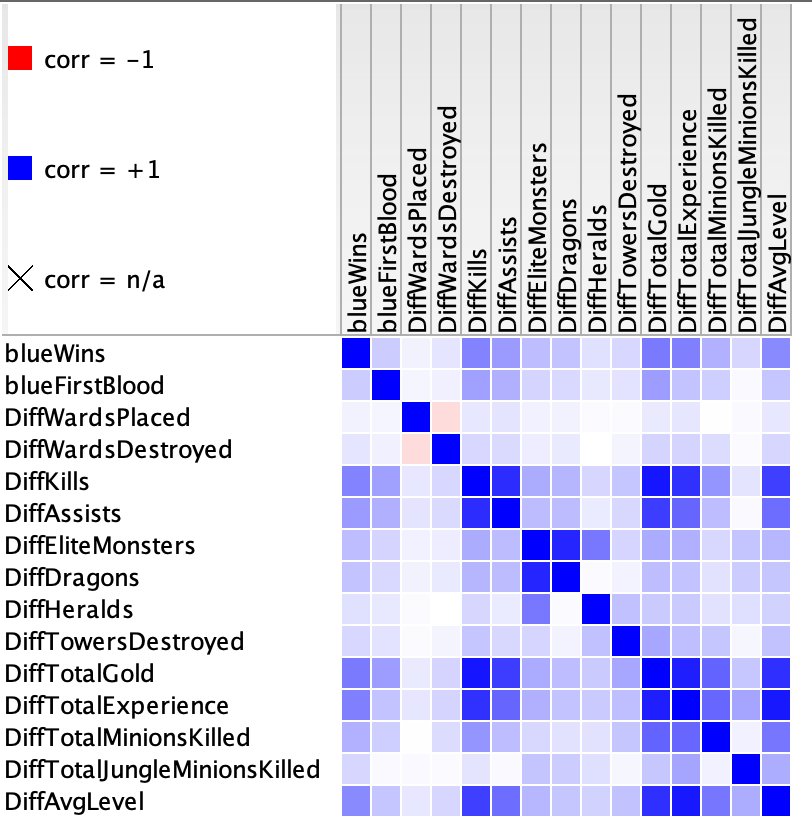
\includegraphics[width=0.5\linewidth]{Figures/RankCorrelation.png}
    \caption{Correlação entre features após processamento.}
    \label{fig:corr1}
\end{figure}

Pela figura \ref{fig:corr1} conseguimos detetar algumas correlações menos óbvios do que obtidas anteriormente. Por exemplo, podemos observar que a diferença em kills está fortemente correlacionada positivamente à diferença em ouro entre as duas equipas.

\begin{figure}[H]
    \centering
    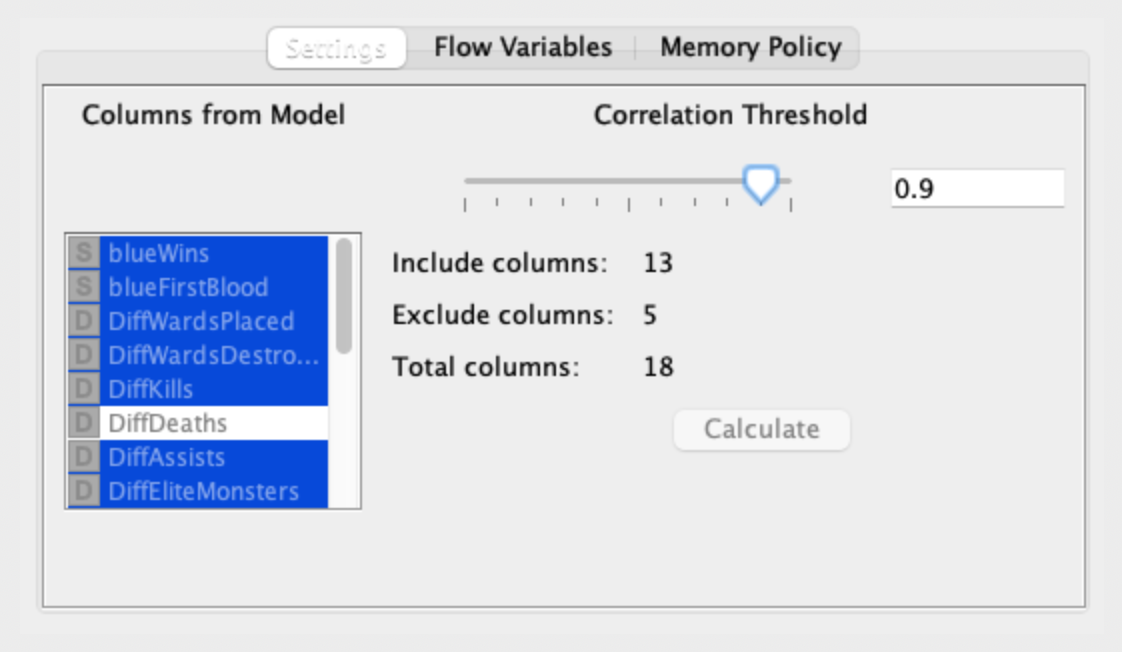
\includegraphics[width=0.5\linewidth]{Figures/Screenshot_2020-11-25_at_22.10.32.png}
    \caption{Seleção automática de features correlacionadas.}
    \label{fig:corr2}
\end{figure}


Como é desnecessário considerar atributos fortemente correlacionados entre si, utilizamos um correlation filter com as configurações da figura \ref{fig:corr2}.

% STEP 4 IN CRISP DM METODOLOGY
\subsection{Modelação}
De forma a garantir a ausência de overfitting decidimos que o ideal seria considerar um modelo baseado em \textit{random forest} que, devido à sua aleatoriadade, permite reduzir fortemente o overfitting.

Com métodos auxiliares de hyper-parameter tuning, fomos capazes de descobrir os hyper-parâmetros ideias para o nosso problema e re-aplicar esses parâmetros directamente na previsão do nosso test set, obtendo uma accuracy perto de 73\%, como se verifica em capítulos adiante. 

% STEP 5 IN CRISP DM METODOLOGY
\subsection{Apreciação dos Modelos}
Utilizando \textit{cross validation} com 10 \textit{folds}, foi possível chegar à conclusão de que a \textit{accuracy} do nosso modelo tende a rondar os 92\% que é, de longe, muito melhores que os nossos modelos iniciais, onde a \textit{accuracy} rondava sempre os 88-89\%. Como tal, este modelo foi seleccionado para ser submetido.